\documentclass[../../main.tex]{subfiles}

\begin{document}
\section{Mutual Information}
\subsection{Exponential Decay in Markov Chains}
    \noindent
    If we have a Markov chain defined by the matrix $\boldsymbol{M}$ (we adopt the notation in the paper and write $\bm{M}$ instead of $\bm{P}$), which is \emph{irreducible} and \emph{aperiodic}, and has a finite state space $S = \{1, \dots, n\}$, then we have that
    \[
        \lim_{i \to \infty} \boldsymbol{M}^i = \boldsymbol{M}_{\boldsymbol{\mu}} \quad ,
    \]
    where $\boldsymbol{M_\mu}$ is the matrix whose columns all consist of the unique stationary probability distribution $\boldsymbol{\mu}$.

    ~\\
    Now, let us consider two random variables $X$ and $Y$, which will denote the state of the Markov chain at times $t_0$ and $t_0 + \tau$ respectively. We assume that we measure these variables very late in the process, where we already have that $\boldsymbol{M}^{t_0} \approx \boldsymbol{M}_{\boldsymbol{\mu}}$. We will use this "equality" later.

    ~\\
    Our goal now is to quantify the mutual information of $X$ and $Y$, that is, the discrepancy between the joint probability distribution $P(X, Y)$ and the one defined by the product of the two marginalized distributions, that is $P'(X, Y) \coloneqq P(X) \cdot P(Y)$. We use the Kullback-Leibler divergence, so our target expression becomes
    \[
        D(P(X, Y) \,\|\, P'(X, Y)) \quad .
    \]

    \smallskip \noindent
    Note that of course this divergence $I(X, Y) \coloneqq D(P(X, Y) \,\|\, P'(X, Y))$ depends on the properties of $M$, as well as on $\tau$. Because $\boldsymbol{M}$ is irreducible and aperiodic, it follows that $|\lambda_2| < 1$. The claim is that
    \[
        I(X, Y) \in \mathcal{O}(|\lambda_2|^\tau) \quad .
    \]
    
    \bigskip \noindent
    There is a lot of math involved, so let us first get an intuition for what is going on. When considering Markov chains, we consider a set of states, say $S = \{A, B, C\}$, and for each time $t \in \mathbb{N}$ we assign a probability to the random variable $X_t \in S$. So let us consider the following Markov chain in figure~\ref{fig:markov_chain}.

    \begin{figure}[h]
    \center
    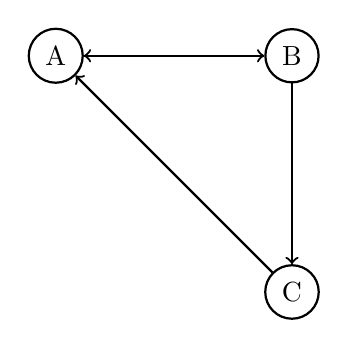
\begin{tikzpicture}[->, auto, node distance=3cm, thick]
    % Define states
    \node[circle, draw] (A) {A};
    \node[circle, draw, right of=A] (B) {B};
    \node[circle, draw, below of=B] (C) {C};

    % Transitions between states
    \draw (A) edge (B);
    \draw (B) edge (A);
    \draw (B) edge (C);
    \draw (C) edge (A);

    % Self-loops
    % \draw (A) edge[loop above] (A);
    % \draw (B) edge[loop above] (B);
    % \draw (C) edge[loop below] (C);

    \end{tikzpicture}
    \caption{A simple irreducible aperiodic Markov chain. Note that if $X_{t_0} = C$, then we know that $X_{t_0+1} = A$.}
    \label{fig:markov_chain}
    \end{figure}

    \noindent
    If $\tau = 1$, i.e. we consider the mutual information of to consecutive states, we get a large value of $I(X, Y)$, as if $X_{t_0}$ is either $A$ or $C$, then $X_{t_0+1}$ is uniquely determined, so we have a strong dependency between the two random variables. If, however, we have $\tau = 5$, then we can reach every state independent of the starting position. To see this, note that we can reach every state from $A$ in four steps:
    \begin{itemize}
        \item $A \rightarrow B \rightarrow C \rightarrow A \rightarrow B$
        \item $A \rightarrow B \rightarrow A \rightarrow B \rightarrow C$
        \item $A \rightarrow B \rightarrow A \rightarrow B \rightarrow A$
    \end{itemize}
    The last step can then be used to go around in a cycle. If we on the other hand started at $B$ or $C$, then we could go to $A$ in one step, and consequently to every other state in the following four. Hence, the probability distribution will "wash out" over time and converge to the stationary one, which results in a decline of $I(X, Y)$ for increasing $\tau$.
    
    ~\\
    Because we measure our $X$ very late in time, meaning $t_0$ is very large, we will have that $P(X = a) \approx \boldsymbol{\mu}_a$ because of this "washing out". Similarly, we have $P(Y = b) \approx \boldsymbol{\mu}_b$, since the probability distribution will only get attracted more towards $\boldsymbol{\mu}$. As we now increase $\tau$, $P(Y = b \,|\, X = a)$ itself will converge to $\boldsymbol{\mu}_b$ exactly due to the same "washing out" reason. Note that $P(Y = b \,|\, X = a) = (\boldsymbol{M}^{\tau})_{ba} \xrightarrow{\tau \to \infty}  \boldsymbol{\mu}_b$. And, of course, if $P(X = a, Y = b) = P(X = a) \cdot P(Y = b \,|\, X = a) = \boldsymbol{\mu}_a \cdot \boldsymbol{\mu}_b$, we have $I(X, Y) = 0$. Hence, in a sense the theorem describes how fast $\boldsymbol{M}^{\tau}\bm{p}_0$ converges to $\boldsymbol{\mu}$, or, equivalently, $\boldsymbol{M}^{\tau}$ towards $\boldsymbol{M}_{\boldsymbol{\mu}}$.

    \bigskip \bigskip \noindent
    Now it's time to dive into the math. In the following, we try to reconstruct the arguments given in the paper. We also adopt the notation $P (a, b) \equiv P (X = a, Y = b)$. By definition of the Kullback-Leibler divergence, we have
    \begin{align*}
        D(P(X, Y) \,\|\, P'(X, Y)) &= \sum_{(a,b) \in S^2} P(a, b) \log_B \frac{P(a, b)}{P(a) P(b)} \quad .
    \end{align*}
    The idea is now that $log_B(\bullet)$ is \emph{concave}. Hence, we can upper bound it by its Taylor expansion of the first degree at the point $x_0 = 1$:
    \begin{align*}
        \log_B(x) &\leq \log_B(x_0) + \log_B'(x_0) (x - x_0) \\
        &= 0 + \frac{\ln'(x_0)}{\ln(B)} (x - 1) \\
        &= \frac{\frac{1}{x_0}}{\ln(B)} (x - 1) \\
        &= \frac{x - 1}{\ln(B)} \quad .
    \end{align*}
    For simplicity, we set $B \coloneqq e$. So our expression becomes
    \begin{align*}
        D(P(X, Y) \,\|\, P'(X, Y)) &\leq \frac{1}{\ln(B)}\sum_{(a,b) \in S^2} P(a, b) \left( \frac{P(a, b)}{P(a) P(b)} - 1 \right) \\
        &= \sum_{(a,b) \in S^2} P(a, b) \left( \frac{P(a, b)}{P(a) P(b)} - 1 \right) \\
        &= \left( \sum_{(a,b) \in S^2} P(a, b) \frac{P(a, b)}{P(a) P(b)} \right) - 1 \\
        &= \left( \sum_{(a,b) \in S^2} \frac{P(a, b)^2}{P(a) P(b)} \right) - 1 \\
        &\eqqcolon I_R(X, Y) \quad .
    \end{align*}
    The authors of the paper coin this definition for $I_R(X, Y)$ the \emph{rational mutual information}, as it has some useful properties. As discussed, we can approximate $P(a) \approx \boldsymbol{\mu}_a$ and $P(b) \approx \boldsymbol{\mu}_b$, and also $P(b \,|\, a) = (\boldsymbol{M}^{\tau})_{ba}$. Thus:
    \begin{align*}
        I_R(X, Y) + 1 &= \sum_{(a,b) \in S^2} \frac{P(a, b)^2}{P(a) P(b)} \\
        &= \sum_{(a,b) \in S^2} \frac{P(b \,|\, a)^2 P(a)^2}{P(a) P(b)} \\
        &= \sum_{(a,b) \in S^2} \frac{\boldsymbol{\mu}_a}{\boldsymbol{\mu}_b} \left[ (\boldsymbol{M}^{\tau})_{ba} \right] ^2 \quad .
    \end{align*}
    Let us now focus on $(\boldsymbol{M}^{\tau})_{ba}$. For simplicity, we consider the case that $\boldsymbol{M}$ is diagonalizable. Note that since M is irreducible and aperiodic, we have that $1 = \lambda_1 > |\lambda_2| \geq \dots \geq |\lambda_n|$. The authors provide proof for the other case as well. But for now, let
    \[
        \boldsymbol{M} = \boldsymbol{BDB}^{-1}
    \]
    be the diagonalization of $\boldsymbol{M}$. Of course, we immediately see that $\boldsymbol{M}^\tau = \boldsymbol{BD}^\tau \boldsymbol{B}^{-1}$. Hence, it is easy to verify that
    \[
        (\boldsymbol{M}^\tau)_{ba} = \sum_{c = 1}^{n} \lambda_c^\tau \boldsymbol{B}_{bc}(\boldsymbol{B}^{-1})_{ca} \quad .
    \]

    \bigskip \noindent
    Okay, that was a lot of math. Now it is a good time to reassure ourselves what we actually have achieved. What do we expect $(\boldsymbol{M}^\tau)_{ba}$ to look like for $\tau \rightarrow \infty$? $\boldsymbol{\mu}_b$ of course. What does $\boldsymbol{B}$ look like? Well, this is very hard to tell, it at least should have a scaled version of $\boldsymbol{\mu}$ in its first column. But we cannot really infer any information about $\boldsymbol{B}^{-1}$. But we know
    \begin{align*}
        \boldsymbol{\mu}_b &= \lim_{\tau \to \infty} (\boldsymbol{M}^\tau)_{ba} \\
        &= \lim_{\tau \to \infty} \sum_{c = 1}^{n} \lambda_c^\tau \boldsymbol{B}_{bc}(\boldsymbol{B}^{-1})_{ca} \\
        &= \lambda_1 \boldsymbol{B}_{b1}(\boldsymbol{B}^{-1})_{1a} \quad .
    \end{align*}
    So we know that
    \[
        (\boldsymbol{M}^\tau)_{ba} = \boldsymbol{\mu}_b \pm \mathcal{O}(|\lambda_2|^\tau) \quad .
    \]
    Note that this is informal writing. It would be more precise to state that $|(\boldsymbol{M}^\tau)_{ba} - \boldsymbol{\mu}_b| \in \mathcal{O}(|\lambda_2|^\tau)$.

    ~\\
    This is looking promising, as this means that the discrepancy between $(\boldsymbol{M}^\tau)_{ba}$ and $\boldsymbol{\mu}_b$ decays exponentially. The only thing left to do is translating this exponential decay to the mutual independence measure $I_R(X, Y)$. To this end, we plug our results back into our previous equation. Note that this step deviates from the procedure in the paper (own interpretation, informal!). Thus:
    \begin{align*}
        I_R(X, Y) &= \left( \sum_{(a,b) \in S^2} \frac{\boldsymbol{\mu}_a}{\boldsymbol{\mu}_b} \left[ (\boldsymbol{M}^{\tau})_{ba} \right] ^2 \right) - 1 \\
        &= \sum_{(a,b) \in S^2} \left( \frac{\boldsymbol{\mu}_a}{\boldsymbol{\mu}_b} \left[ (\boldsymbol{M}^{\tau})_{ba} \right] ^2 - \boldsymbol{\mu}_a \boldsymbol{\mu}_b \right) \\
        &= \sum_{(a,b) \in S^2} \left( \frac{\boldsymbol{\mu}_a}{\boldsymbol{\mu}_b} \left[ \boldsymbol{\mu}_b \pm \mathcal{O}(|\lambda_2|^\tau) \right] ^2 - \boldsymbol{\mu}_a \boldsymbol{\mu}_b \right) \\
        &= \sum_{(a,b) \in S^2} \left( \frac{\boldsymbol{\mu}_a}{\boldsymbol{\mu}_b} \left[ \boldsymbol{\mu}_b^2 \pm \mathcal{O}(|\lambda_2|^\tau) \right] - \boldsymbol{\mu}_a \boldsymbol{\mu}_b \right) \\
        &= \pm \sum_{(a,b) \in S^2} \frac{\boldsymbol{\mu}_a}{\boldsymbol{\mu}_b} \mathcal{O}(|\lambda_2|^\tau) \quad , \\
    \end{align*}
    where we have used multiple facts about $\boldsymbol{\mu}$. For instance, $\sum_{a \in S} \boldsymbol{\mu}_a = 1$ and thus $\sum_{(a,b) \in S^2} \boldsymbol{\mu}_a \boldsymbol{\mu}_b = 1$, as well as $0 < \boldsymbol{\mu}_a < 1$ for all $a \in S$ (at least for $|S| > 1$). We now use the latter inequality again: We see that we can always bound $\frac{\boldsymbol{\mu}_a}{\boldsymbol{\mu}_b}$ from above, i.e. there exists $\alpha \in \mathbb{R}$ s.t. for all $(a,b) \in S^2$ we have $\frac{\boldsymbol{\mu}_a}{\boldsymbol{\mu}_b} < \alpha$. Hence:

    \begin{align*}
        &|I_R(X, Y)| \in \sum_{(a,b) \in S^2} \frac{\boldsymbol{\mu}_a}{\boldsymbol{\mu}_b} \mathcal{O}(|\lambda_2|^\tau) \\
        &\implies |I_R(X, Y)| \in \sum_{(a,b) \in S^2} \alpha \mathcal{O}(|\lambda_2|^\tau) \\
        &\implies |I_R(X, Y)| \in n^2 \alpha \mathcal{O}(|\lambda_2|^\tau) \\
        &\implies |I_R(X, Y)| \in \mathcal{O}(|\lambda_2|^\tau) \quad .
    \end{align*}
    Of course, $I_R(X, Y) \geq 0$, so really $I_R(X, Y) \in \mathcal{O}(|\lambda_2|^\tau)$. Since $0 \leq I(X, Y) \leq I_R(X, Y)$, we also have $I(X, Y) \in \mathcal{O}(|\lambda_2|^\tau)$.

    \bigskip
    \begin{remark}
        Based on the proof, we see that if the distance between $\bm{M}^\tau$ and $\bm{M_\mu}$ experiences exponential decay, we can translate this exponential decay to the mutual information measure $I_R(X, Y)$. Note that we have already established that irreducible aperiodic Markov chains have this property in remark~\ref{remark:exponential_decay}.
    \end{remark}

\subsection{The Degenerate Case}
    Nonetheless, we will prove the case that $\bm{M}$ is not diagonalizable seperately and establish the connection to $\lambda_2$.
\end{document}